\section{State of Art}
\subsection{Definitions}
In this subsection, definitions about the graph theory will be presented. Most of the following definitions are taken from or inspired by wikipedia and wikibook.
\subsubsection{Type of graphs}
\paragraph{Undirected graphs :}
Undirected graphs are mathematical objects composed of a set of vertices $V$
and a set of edges $E$ and are noted $G = (V,E)$.

\paragraph{}
Also called nodes, vertices are mathematical objects which might virtually
represent anything, a vertices is usually noted $v$.

\paragraph{}
Edges are an unordered pair of vertices noted $e = \{u,v\}$. Edges might
contain twice the same vertex, in this case, the edge is called a {\em loop}.

\begin{figure}[!h]
  \begin{center}
    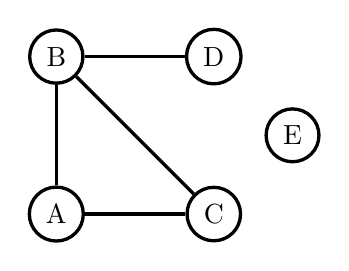
\begin{tikzpicture}[scale=0.5]
  \node[draw,circle, very thick] (A) at (2,0) {A};
  \node[draw,circle, very thick] (B) at (2,4) {B};
  \node[draw,circle, very thick] (C) at (6,0) {C};
  \node[draw,circle, very thick] (D) at (6,4) {D};
  \node[draw,circle, very thick] (E) at (8,2) {E};
  \draw[very thick] (A) -- (B);
  \draw[very thick] (B) -- (D);
  \draw[very thick] (C) -- (B);
  \draw[very thick] (C) -- (A);
\end{tikzpicture}

  \end{center}
  \caption{An undirected simple graph with 5 vertices and 4 edges}
\end{figure}

\paragraph{Directed graphs :} 
A directed graph is a graph with edge define as and ordered pairs $e = (u,v)$ rather than a two-element set $e = \{u,v\}$.
\begin{figure}[!h]
  \begin{center}
    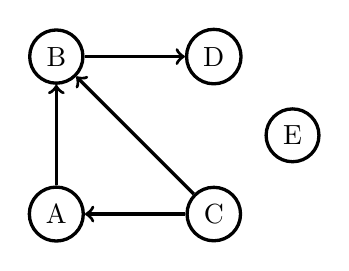
\begin{tikzpicture}[scale=0.5]
 \tikzset{directed/.style={->}} 
  \node[draw,circle, very thick] (A) at (2,0) {A};
  \node[draw,circle, very thick] (B) at (2,4) {B};
  \node[draw,circle, very thick] (C) at (6,0) {C};
  \node[draw,circle, very thick] (D) at (6,4) {D};
  \node[draw,circle, very thick] (E) at (8,2) {E};
  \draw[very thick, directed] (A) -- (B);
  \draw[very thick, directed] (B) -- (D);
  \draw[very thick, directed] (C) -- (B);
  \draw[very thick, directed] (C) -- (A);
\end{tikzpicture}

  \end{center}
  \caption{A directed simple graph with 5 vertices and 4 edges}
\end{figure}

\paragraph{Subgraphs :}
Given a graph $G = (V,E)$ and a graph $G' = (V',E')$, $G'$ is a subgraph of $G$ if and only if $V \subseteq V'$ and $E \subseteq E'$.

\begin{figure}[!h]
  \begin{center}
    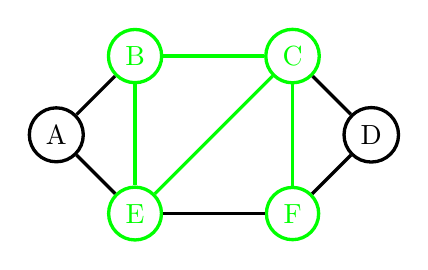
\begin{tikzpicture}[scale=0.5]
  \node[draw,circle, very thick] (A) at (0,2) {A};
  \node[draw,circle, very thick, color=green] (B) at (2,4) {B};
  \node[draw,circle, very thick, color=green] (C) at (6,4) {C};
  \node[draw,circle, very thick] (D) at (8,2) {D};
  \node[draw,circle, very thick, color=green] (E) at (2,0) {E};
  \node[draw,circle, very thick, color=green] (F) at (6,0) {F};
  \draw[very thick] (A) -- (B);
  \draw[very thick] (A) -- (E);
  \draw[very thick, color=green] (B) -- (C);
  \draw[very thick, color=green] (B) -- (E);
  \draw[very thick] (C) -- (D);
  \draw[very thick, color=green] (C) -- (E);
  \draw[very thick, color=green] (C) -- (F);
  \draw[very thick] (D) -- (F);
  \draw[very thick] (E) -- (F);
\end{tikzpicture}

  \end{center}
  \caption{A graph and one of his subgraph}
\end{figure}

\paragraph{Tree :}
A tree is an undirected graph without cycles,

\begin{figure}[!h]
  \begin{center}
    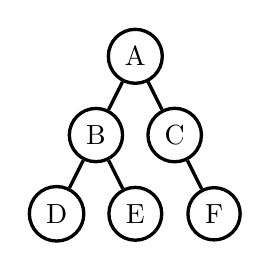
\begin{tikzpicture}[scale=0.5]
  \node[draw,circle, very thick] (A) at (2,4) {A};
  \node[draw,circle, very thick] (B) at (1,2) {B};
  \node[draw,circle, very thick] (C) at (3,2) {C};
  \node[draw,circle, very thick] (D) at (0,0) {D};
  \node[draw,circle, very thick] (E) at (2,0) {E};
  \node[draw,circle, very thick] (F) at (4,0) {F};
  \draw[very thick] (A) -- (B);
  \draw[very thick] (A) -- (C);
  \draw[very thick] (B) -- (D);
  \draw[very thick] (B) -- (E);
  \draw[very thick] (C) -- (F);
\end{tikzpicture}

  \end{center}
  \caption{A tree}
\end{figure}

\paragraph{Spanning Tree :}
A tree is a spanning tree of a graph G if it includes every vertex of G and is a subgraph of G (every edge in the tree belongs to G).

\begin{figure}[!h]
  \begin{center}
    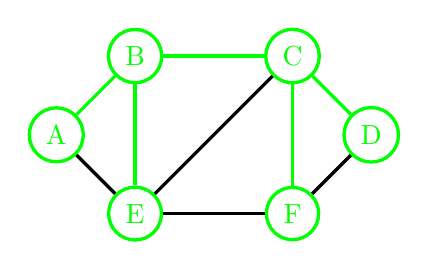
\begin{tikzpicture}[scale=0.5]
  \node[draw,circle, very thick, color=green] (A) at (0,2) {A};
  \node[draw,circle, very thick, color=green] (B) at (2,4) {B};
  \node[draw,circle, very thick, color=green] (C) at (6,4) {C};
  \node[draw,circle, very thick, color=green] (D) at (8,2) {D};
  \node[draw,circle, very thick, color=green] (E) at (2,0) {E};
  \node[draw,circle, very thick, color=green] (F) at (6,0) {F};
  \draw[very thick, color=green] (A) -- (B);
  \draw[very thick] (A) -- (E);
  \draw[very thick, color=green] (B) -- (C);
  \draw[very thick, color=green] (B) -- (E);
  \draw[very thick, color=green] (C) -- (D);
  \draw[very thick] (C) -- (E);
  \draw[very thick, color=green] (C) -- (F);
  \draw[very thick] (D) -- (F);
  \draw[very thick] (E) -- (F);
\end{tikzpicture}

  \end{center}
  \caption{A spanning tree}
\end{figure}

\subsubsection{Fundamentals notations}
\paragraph{Graph Size :}
The size of a graph is the number of edges it contains and is noted
$m = |E|$.

\paragraph{Graph order :}
The order of a graph is the number of vertices it contains and is noted
$n = |V|$.

\paragraph{Vertex degree :}
The degree of a vertex is equal to the number of edges incident to it, loops
are counted twice.

\subsubsection{Path}
\paragraph{Path :}
A path of length $n$ is a sequence of alternated vertices and edged, noted
$P = \{v_0, e_1, v_1, e_2, ..., e_n, v_n\}$ such as :
$\forall i \in \{1,2, ..., n\}, e_i = \{v_i, v_{i-1}\}$. If $v_0 = v_n$, $P$ is
a cycle.

\begin{figure}[!h]
  \begin{center}
    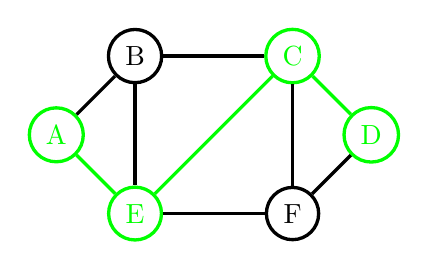
\begin{tikzpicture}[scale=0.5]
  \node[draw,circle, very thick, color=green] (A) at (0,2) {A};
  \node[draw,circle, very thick] (B) at (2,4) {B};
  \node[draw,circle, very thick, color=green] (C) at (6,4) {C};
  \node[draw,circle, very thick, color=green] (D) at (8,2) {D};
  \node[draw,circle, very thick, color=green] (E) at (2,0) {E};
  \node[draw,circle, very thick] (F) at (6,0) {F};
  \draw[very thick] (A) -- (B);
  \draw[very thick, color=green] (A) -- (E);
  \draw[very thick] (B) -- (C);
  \draw[very thick] (B) -- (E);
  \draw[very thick, color=green] (C) -- (D);
  \draw[very thick, color=green] (C) -- (E);
  \draw[very thick] (C) -- (F);
  \draw[very thick] (D) -- (F);
  \draw[very thick] (E) -- (F);
\end{tikzpicture}

  \end{center}
  \caption{A path of length 4}
\end{figure}

\subsubsection{Cuts}
Let $G=(V,E)$ be a graph.
\paragraph{Cut :}
A cut $C=(S,T)$ is a partition of $V$ into two disjoint subsets that are joined by at least one edge.

\paragraph{Cut-set :}
The cut-set of a cut $C=(S,T)$ is the set of edge defined as $\{(u,v)\in E | u\in S, v \in T\}$.

\paragraph{Cut size :}
The size of a cut is the number of edges in the cut-set.


\begin{figure}[!h]
  \begin{center}
    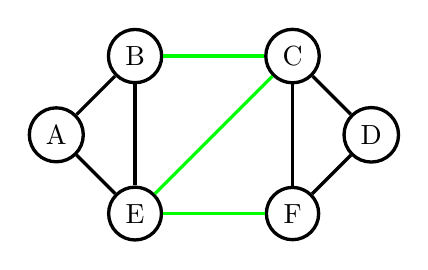
\begin{tikzpicture}[scale=0.5]
  \node[draw,circle, very thick] (A) at (0,2) {A};
  \node[draw,circle, very thick] (B) at (2,4) {B};
  \node[draw,circle, very thick] (C) at (6,4) {C};
  \node[draw,circle, very thick] (D) at (8,2) {D};
  \node[draw,circle, very thick] (E) at (2,0) {E};
  \node[draw,circle, very thick] (F) at (6,0) {F};
  \draw[very thick] (A) -- (B);
  \draw[very thick] (A) -- (E);
  \draw[very thick, color=green] (B) -- (C);
  \draw[very thick] (B) -- (E);
  \draw[very thick] (C) -- (D);
  \draw[very thick, color=green] (C) -- (E);
  \draw[very thick] (C) -- (F);
  \draw[very thick] (D) -- (F);
  \draw[very thick, color=green] (E) -- (F);
\end{tikzpicture}

  \end{center}
  \caption{A cut-set in green}
\end{figure}

\paragraph{Minimun cut :} 
The minimun cut is the cut with the lowest size. 

\subsubsection{Flow}
\paragraph{Flow :}
%TODO

\paragraph{Maximun-flow Minimun-cut Theorem :}
%TODO


\subsubsection{Connectivity}
\paragraph{Connectivity :}
A graph  is {\em connected} if $\forall u,v \in V$ a path exists from $u$
to $v$. Otherwise, the graph is {\em unconnected}

\paragraph{k-connectivity :}
A graph with a least two vertices is k-connected if, for every pair of vertices, there is at least k vertex disjoint paths between these vertices.

Another definitions could be, a graph is k-connected if the smallest subset which disconnect the graph if you delete it is of size k.

\begin{figure}[!h]
  \begin{center}
    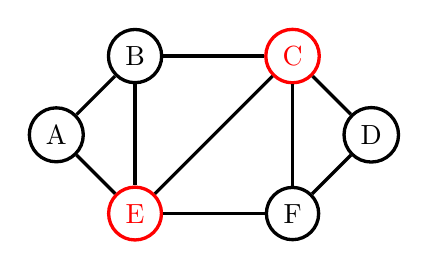
\begin{tikzpicture}[scale=0.5]
  \node[draw,circle, very thick] (A) at (0,2) {A};
  \node[draw,circle, very thick] (B) at (2,4) {B};
  \node[draw,circle, very thick, color=red] (C) at (6,4) {C};
  \node[draw,circle, very thick] (D) at (8,2) {D};
  \node[draw,circle, very thick, color=red] (E) at (2,0) {E};
  \node[draw,circle, very thick] (F) at (6,0) {F};
  \draw[very thick] (A) -- (B);
  \draw[very thick] (A) -- (E);
  \draw[very thick] (B) -- (C);
  \draw[very thick] (B) -- (E);
  \draw[very thick] (C) -- (D);
  \draw[very thick] (C) -- (E);
  \draw[very thick] (C) -- (F);
  \draw[very thick] (D) -- (F);
  \draw[very thick] (E) -- (F);
\end{tikzpicture}

  \end{center}
  \caption{A 2-connected graphe}
\end{figure}

\paragraph{Menger's theorem :}
The menger's theorem is an important theorem concerning connectivity.
It states the following fact:

Let G be a undirected graph and a and b two distinct vertices.
Then the size of the minimun edge cut for a and b is equal to the maximun number of pairwise node-independent paths from a to b.


\subsubsection{Partition}
\paragraph{k-partition :}
A set $\{V_1,...,V_k\}$ is a k-partition:
\begin{itemize}
    \item $\forall i, \lceil V_i \rceil$ is connected
    \item $\sum\limits_{i=0}^k|V_i| = |V|$
    \item $\forall i,j \in \{1, \dots, k\}^2, i \neq j, V_i \cap V_j = \emptyset$
\end{itemize}

\begin{figure}[!h]
    \begin{center}
        
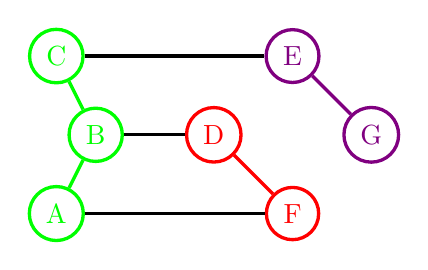
\begin{tikzpicture}[scale=0.5]
  \node[draw,circle, very thick, color=green] (A) at (0,0) {A};
  \node[draw,circle, very thick, color=green] (B) at (1,2) {B};
  \node[draw,circle, very thick, color=green] (C) at (0,4) {C};
  \node[draw,circle, very thick, color=red] (D) at (4,2) {D};
  \node[draw,circle, very thick, color=violet] (E) at (6,4) {E};
  \node[draw,circle, very thick, color=red] (F) at (6,0) {F};
  \node[draw,circle, very thick, color=violet] (G) at (8,2) {G};
  \draw[color=green, very thick] (A) -- (B);
  \draw[color=green, very thick] (B) -- (C);
  \draw[very thick] (B) -- (D);
  \draw[very thick] (A) -- (F);
  \draw[very thick] (C) -- (E);
  \draw[very thick, color=violet] (E) -- (G);
  \draw[very thick, color=red] (D) -- (F);
\end{tikzpicture}

    \end{center}
    \caption{A 3-partition graph}
\end{figure}

\subsection{Algorithme}
\subsubsection{k-connectivity}
\paragraph{}
As we have seen in the previuos section, the connectivty of a graph is equal to the size of the smallest subset wich disconnect the graph.
To do so the max-flow min-cut theorem states that the maximun flow between to vertices is equal to the minimun cut to disconect this to vertices.
But if we use directly a flow algorithm, we will compute the edge-connectivity and not the vertex-connectivity.

So first the graph need to be transform. We need capacity on the nodes. To do so each nodes will be divided into two new nodes. Each incomming edge will be attach to the first node and each leaving edge to the second node. Another edge will be add between the two new node.
The capacity of all edge of the graph will be set to 1.

Then to find the connectivity, we compute the maximun flow between each pair of nodes and we keep only the lowest value. This value is the connecivity.


\begin{algorithm}[!h]
    \KwData{$G=(V,E)$ a graph}
    \KwResult{$k$ the connecitvity}
    $min = \infty$\;
    $G^{'} = TransformNode(G)$\;
    \ForAll{$u,v \in V, u \neq v, (u,v) \notin E$}{
        $f = maximunFlow(G^{'},u,v)$\;
        \If{$f < min$}{
            $min = f$\;
    }
}
    \Return{$min$}\;
    \caption{Compute the connecitvity}
\end{algorithm}

%TODO write pseudo-algorithm
% min = inf
% For each pair of nodes
%   f = Compute the maximun flow
%   If f < min
%       min = f
% return min 
%

